\chapter{Transport mode application to heavy-flavor evolution}
In this chapter, we shall start to focus on applying the LIDO transport model to the heavy-flavor section, and discuss in detail how a transport model fits into the complex dynamics of heavy flavors in the heavy-ion collision environment.

Heavy flavor is a charming probe for the medium created in heavy-ion collisions. 
Its large mass guarantees an negligible thermal production contribution at least for present LHC top beam energies for heavy-ion program (there are estimates that thermal contribution can play a row in future FCC collider).
Therefore, heavy flavors are almost always created in initial hard processes. 
The sparse population of open heavy flavor in the collision also suppresses the chances that they annihilates / recombine with their anti-particles (unless one focus on the production of the quarkonium themselves).
Certainty heavy mesons have a long life time such that the decay vertices are outside the fireball and can be resolved by experiments.
Therefore, the number of heavy-flavor particles is almost conserved and experienced the entire medium evolution including both the QGP phase and the hadronic phase.

Heavy flavor has a rich variety of physics interests. 
At high $p_T$, the evolution of heavy flavor particles merges into the context of jet dynamics and jet energy loss study; at intermediate $p_T$ the mass hierarchy predicted for the medium modifications;
and low $p_T$, heavy flavor is one of the key messengers for the thermalization processes inside QGP due to its long relaxation time compared to light partons.
Charm quark ($M=1.3$ GeV) and bottom quark (M=$4.2$ GeV) are the most relevant heavy quarks for the present study.
The reason that top quark ($173$ GeV) is out of our discussion is due to its extremely short life time ($\sim 5\times 10^{-25} \approx 0.15$  fm/$c$ in its rest frame) so it barely interacts with the QGP before it decays predominantly into bottom quarks.
Though there has also been proposal for taking advantage of this short life-time to probe the temporal structure of the QGP in its early stages, we shall focus on the charm and bottom flavor in this thesis.

We summarize a comprehensive simulation framework for heavy quarks in relativistic heavy-ion collisions in the following follow chart figure \ref{fig:flowchart}.
The soft initial condition model provide both the initial energy density of the medium and the transverse location of the hard vertices, while pQCD based calculations initialize the momentum space of the hard partons.
We have introduced the left branch of this flow chart, which is the hydrodynamic-based model for the bulk medium evolution.
The right branch is a model for the hard parton (heavy flavor) evolution.

Immediately after the hard production, the parton undergoes DGLAP evolution and builds a parton shower.
In fact many heavy flavor particles are created in parton shower stage.
The complication is that certain vacuum parton shower would have occupied the same phase-space as the medium-induced radiation.
One of the many obstacles in interfacing these two processes is that the multiple emissions / branchings are treated very differently between vacuum evolution and in-medium evolution.
For the vacuum evolution, the ``time'' variable is the virtuality scale with the space-time information integrated out, while the transport model evolves the systems in real time, with virtuality integrated out below a certain scale.
There are many recent progress in both theory developments and newly design event-generators to solve this problem.
In this chapter, we shall focus on one possible solution to interface the two in section 1.
The in medium propagation of parton requires the medium properties as input. 
To zeros order of approximation, we specify the medium with its flow velocity and the equilibrium temperature, although the viscous hydro provides far more off-equilibrium information. 
This is discussed in section 2.
The heavy flavor hadronization model is introduced in section 3, which is a previously developed model that interpolates high-$p_T$ fragmentation processes and low-$p_T$ in medium recombination production of heavy hadrons.
In section 4, we briefly introduced how this simulation framework of open heavy flavor can be coupled to the quarkonium evolution, but for more details, please refers to the thesis work [].
Finally, in section 5, we benchmark the model using a few choices of fixed coupling constant and running coupling constants before systematically tuned the model to data in the next chapter.
\begin{figure}
\centering
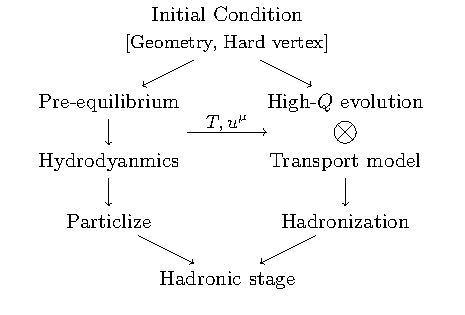
\includegraphics[width=.8\textwidth]{flowchart.pdf}
\caption{hh}
\label{fig:flowchart}
\end{figure}

\section{Initial production of heavy flavor}
\subsection{Factorization framework in proton-proton collisions}
In the proton-proton collision, the hard processes can be computed using the pQCD-based techniques.
The foundation of this calculation is the factorization framework as schematically demonstrated in \ref{fig:factorization}.
First, the incoming proton is a composite object and there is a certain ``probability'' of finding a parton $i(j)$ carrying $x_i(x_j)$ fraction of the momentum of the proton $p_1(p_2)$.
This ``probability'' is known as the parton distribution function (PDF) $f_i(x, Q^2)$.
It not only is a function of $x$, but also depends on the scale $Q^2$ at which the proton is probed.
The probing scale is required to be much greater than the non-perturbative scale.
Because $\alpha_s(Q^2)$ is samll due to asymptotic freedom, perturbative calculation can compute the process of partons $i$ and $j$ scatterings into partons $k$ and $l$.
Finally, the partons produces a bunch of hadrons. 
And one can define a parton fragmentation function as the probability to find a hadron $H$ carrying a fraction $x_H$ of the parton's momentum.
Finally the cross-section for the inclusive production of hadron can be written as [],
\begin{eqnarray}
\frac{d\sigma_{p+p\rightarrow H+X}}{dy d\mathbf{p}_T^2} = \frac{1}{\pi}\int dx_i dx_j f_i(x_i, Q^2) f_j(x_j, Q^2) \frac{d\sigma_{ij\rightarrow kl}}{d\hat{t}} \frac{1}{z_k}D^H(z_k, Q^2).
\end{eqnarray}
Although the parton distribution function $f$ and the parton fragmentation function $D$ are essentially non-perturbative objects and has to be extracted from experiments at certain scales $Q_0^2$, their evolution from $Q_0^2$ to another scale $Q^2$ can be described by the DGLAP evolution equation from perturbative QCD.
This evolution takes into account that the initial high-virtuality parton $i$ (or $j$) could have come from a splitting process of a parton with lower virtuality parton $i'$ (or $j'$).
Similarly, the final state high virtuality parton $k$ (or $l$) could also split into a low virtuality parton $k'$ (or $l'$) before it turns into a hadron.
Though each splitting causes an additional power of $\alpha_s$, it is also magnified by a potentially large factor $\ln Q^2/\mu^2$ when the $Q^2$ is much greater than the scale where the $f$, $D$ are defined.
The same argument also applies to partons $i', j', k', l'$. 
To increase the predictive power of the perturbative calculation, 
the DGLAP equations systematically resum contributions including an arbitrary number of parton splittings and evolve the scale from $\mu^2$ to the hard scale $Q^2$.
Moreover, a very useful parton-shower picture can be built from this process and with a probabilistic interpretation of the DGLAP evolution. Monte Carlo technique, one can mimic the exclusive final states from these sequences of parton branching processes.

\begin{figure}
\centering
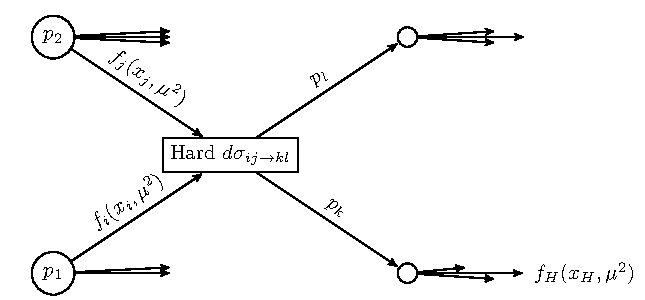
\includegraphics[width=.8\textwidth]{factorization.pdf}
\caption{
}
\label{fig:factorization}
\end{figure}

\subsection{Production in the nuclear environment}
The above framework explains very well explains the hard process production in the proton-proton collisions.
In the nuclear environment, there are several differences.
First, the parton distribution function inside a nuclei is different from the superposition of the nucleons.
The ratio between nuclear PDF and proton PDF generally deviates from unity.
In particular, this ratio for small $x$ gluon is significantly below unity, known as the nuclear shadowing effect. 
For relatively larger $x$, this ratio increase and become larger than one,  termed as the anti-shadowing effect.
The difference between the nuclear PDF and proton PDF belongs is one kind of ``cold nuclear matter'' (CNM) effect, in contrary to the ``hot nuclear matter'' effect from the QGP.
And both needs to be included for a correct interpretation of the experimental data.
The hardest partonic process is not expected to be modified as it happens on a time scale much shorter than that of the medium formation.
However, some of the vacuum parton splittings may have a formation time that overlaps with the medium, and medium effects may modify this phase-space region and this is discussed in the next section.

In the course of my study, I have tried using both the inclusive cross-section program as well as a Monte-Carlo event generator to initialize the heavy quark production in nuclear environment.
\paragraph{Initialize from inclusive cross-section program}
We use FONLL (Fixed-Order-Next-to-Leading-Log) to generate the inclusive production cross-section of heavy flavor at partonic level.
The FONLL program is a combination of the fixed order (NLO) massive matrix-elements and a massless resummation program.
It computes the single inclusive differential cross-section of heavy quark / hadron production $d^2\sigma/dydp_T$.
Then, heavy quark's initial momentum is sampled from $d^2\sigma/dydp_T$.
It has the advantage that it is a first principal calculation when applied to proton-proton collisions, but the main disadvantage is the lack of an exclusive partonic final state.
This causes several problems,
\begin{itemize}
\item[1.] Limit the study to open-heavy flavor.
But for full jet study, one needs the exclusive partonic final state. And for quarkonium study, the momentum correlation among the $Q$-$\bar{Q}$ pairs are important.
\item[2.] We cannot build a space-time picture of the parton shower and cannot implement medium modifications to parton evolution. 
Therefore, it is always assumed that heavy quarks are produced at time $t=0^{+}$ in this initialization choice.
\end{itemize}
\paragraph{Initialize from Monte-Carlo event generator}
Another approach to generate initial hard process is to use high energy Monte-Carlo event generator, such as Pythia [].
Pythia implements the leading order (LO) matrix-elements for hard QCD processes, including LO production of heavy flavor particles,
$g+g\rightarrow Q+\bar{Q}$ and $q+\bar{q}\rightarrow Q+\bar{Q}$.
The parton shower will be generated based on the probabilistic interpretation of the DGLAP equation.
At high energy, the LO production of heavy flavor is only a fraction of the total heavy flavor cross-section, the rest of them are created in the parton showers from the so-called gluon splitting and flavor creation processes.
The former corresponds to a situation where the heavy flavor pair comes from a final state gluon splitting; and the latter produces the pair in initial state gluon splitting and is put-on shell by the hard scattering.
These contributions also mimic certain pair correlations with non back-to-back angular correlations.

This initialization method is not a first principal approach and generate parton shower in high energy collisions can be rather slow, but the benefits are,
\begin{itemize}
\item Though the parton shower in Pythia is evolved as a function of virtuality $Q^2$. 
An approximate space-time picture can be reconstructed by defining the formation time for each branching $2x(1-x)E/k_\perp^2$. Then, it is easy to determine which splitting happened inside the medium and receives medium modification.s
\item Full jet initialization and the study of quarkonium production.
\end{itemize}

\paragraph{A comparison of proton-proton baseline and CNM effect}
We checked whether the pythia event generator prodicts similar proton-proton baseline compared to the first principle approach FONLL.
In the upper plot of figure \ref{fig:pythia-fonll}, we compare the $p_T$ differential cross-section of $p+p\rightarrow c$ from FONLL (lines) and Pythia simulations (symbols), and for Pb+Pb collision (red) and p+p collision (blue) at the LHC energy $\sqrt{s}=5.02$ TeV.
For proton-proton collisions, we use the CT10 parton distribution function [].
The nuclear PDF uses the EPS09 parametrizaiton [].

Though the absolute value of the cross-sections between FONLL and Pythia are different, the interested observables are always ratios between nuclear collisions and the proton-proton baseline where normalization cancels, or other dimensional-less observables such as the momentum-space anisotropy of heavy meson.
Therefore, we focus more on the shape of the spectra between the two calculation, which agree very well.
The ratio of initial charm spectra of Pb+Pb collisions and p+p collisions estimates the magnitude of the cold-nuclear matter effect on the nuclear modification factor $R_{AA}$ (without the hot QGP effect).
FONLL and Pythia simulation predict consistent modulation: the initial production AA spectra of charm quark at low-$p_T$ is suppressed compared to the pp spectra, due to the shadowing effect of the small-$x$ gluon. 
At higher $p_T$, the ratio increase and slightly shoots over unity, because partons from the anti-shadowing contribute more at larger-$x$.

\begin{figure}
\centering
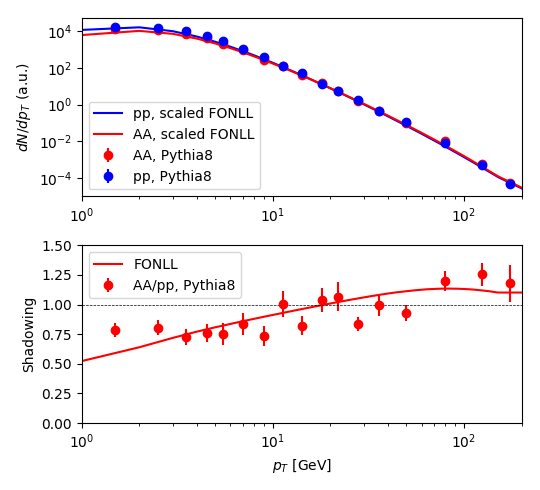
\includegraphics[width=.8\textwidth]{pythia-vs-fonll.png}
\caption{}
\label{fig:pythia-fonll}
\end{figure}

\section{Interfacing vacuum shower with in-medium transport}
\begin{figure}
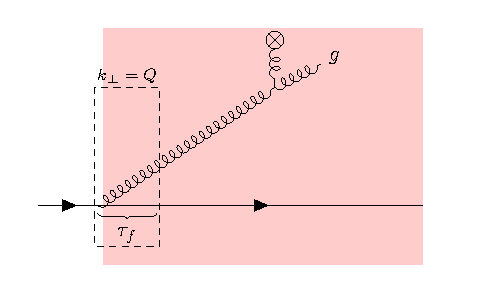
\includegraphics[width=.35\textwidth]{largeQ.pdf}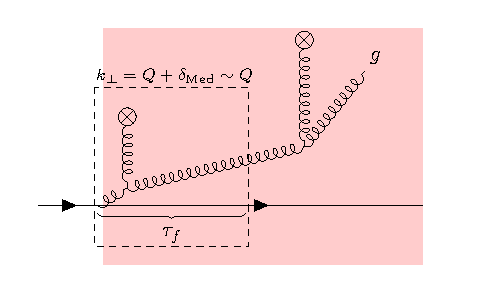
\includegraphics[width=.35\textwidth]{mediumQ.pdf}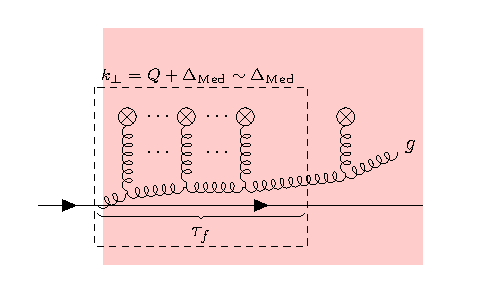
\includegraphics[width=.35\textwidth]{smallQ.pdf}
\caption{}
\label{fig:vac-med-interface}
\end{figure}
Interfacing the vacuum shower that evolves with virtuality and the transport equation that evolves with time is a difficult task. 
We shall provide a reasoning for the prescription we use following a recent development [].

\subsection{A separate treatment of different phase-space}
Considering a vacuum splitting of a hard parton that enters the medium at $z=0$.
The vacuum splitting has formation time $\tau_f \sim 2x(1-x)E/k_\perp^2$.
It is very likely that the radiated gluon (or the quark) interacts with one or more scattering centers (labeled by ``i'') in the medium at time $t_i$.
Whether these interactions contribute coherently to the ``vacuum-like'' splitting follows the same argument as before.
Scatterings that are well separated from the formation processes $\tau_f \ll t_i$ are treated as independently, and it only broadens the transverse momentum without changing the probability of the process.
For $t_i \lesssim \tau_f$, the branching probability of the vacuum-like radiation also gets modified, in addition to broadening.
Now, lets classify a few difference cases using an average ``number'' of scatterings  $N = \tau_f/\lambda$ for the case of a static medium.
\begin{itemize}
\item For a branching with large virtuality (left of figure \ref{fig:vac-med-interface}) so that $N \ll 1$, which translates into $k_\perp^2 \gg  g^2 x(1-x)E T$. 
The chance for the medium modification the vacuum branching probability is negligible. 
\item Hold the energy of the radiaion, while decrease its virtuality (middle of figure \ref{fig:vac-med-interface}) so that $N = \tau_f/\lambda \sim 1$ ($k_\perp^2 \sim g^2 x(1-x)E T$). 
Now, there is an order one probability of scatterings within $\tau_f$, but the transverse momentum of the gluon is still dominated by the initial virtuality.
The probability for the branching should also be modified accordingly, for example, using the higher-twist formula that expanded in terms of $1/k_\perp^2$.
\item Further decreasing the initial virtuality of the branching (right of figure \ref{fig:vac-med-interface}) until $N = \gg 1$,
the medium broadening to the branching eventually dominates over the the virtuality.
And $k_\perp^2 \sim g^2\sqrt{x(1-x)E T^3}$. 
When this happens, the branching probability is heavily modified by the medium and should be replaced by a medium-induced splitting calculation.
\end{itemize}
Summarizing the two extreme regions:
High-virtuality part of the shower $k_\perp^2 \gg \alpha_s \omega T$ is not modified, while low-virtuality part $k_\perp^2 \sim \sqrt{\hat{q}\omega}$ (in a static medium) are replaced by medium-induced radiations.
It is therefore natural to use $k_\perp^2$ and the fraction that is contributed by the medium broadening $\Delta k_\perp^2$ to separate the medium-induced radiation and the vacuum-like radiation.
Since medium induced radiations treated by the transport equation always have $k_\perp^2 = \Delta k_\perp^2$,  our interfacing prescription is then to simply cut-out the vacuum branchings generated by Pythia in the region $k_\perp^2 <  \Delta k_\perp^2$ (this is also known as the vetoed region in the literature []).
For a general medium, $\Delta k_\perp^2$ has to be determined case-by-case for each branchings.
If the medium is finite, then there are also vacuum branchings that formed outside of the medium.
These branchings do not resolve the details of the medium and its probability is not modified.
This separated treatment of different region of phase-space depends on the detailed choice of the separation scale, so in the future, it would be ideal to develop a unified treatment of both vacuum and medium-induced shower in the time evolution picture.

Here, we only concern the modification of the vacuum-like radiation from a heavy quark.
First, in the generated Pythia event, one trace back a heavy quark line to find all the gluons from its final state radiation (FSR) and the original four momentum of the heavy quark at initial production.
These FSR gluons are first treated as ``unformed'' by the transport models, and they are allowed to undergo elastic broadening with the medium.
In this way, by the time these gluons reaches its formation time ($t-t_0>\tau_f$), one knows what is the initial virtuality and of the splitting $k_\perp^2$, as well as how much medium broadening is acquired $\Delta k_\perp^2$.
Then, applying for our previous approximation, vacuum-like branching with 
$k_\perp^2 > \Delta k_\perp^2$ is unmodified, but $k_\perp^2 < \Delta k_\perp^2$ ones are rejected because this contribution is already taken care by the medium-induced rate in the transport model.

\subsection{Visualization on the Lund diagram}
The Lund diagram is useful tool to visualize the separation of phase-space for high energy parton splitting.
There are many different choice of kinematic variables, but here we choose the vertical axis to be $Y = ln(1/x) = \ln(E/\omega)$, and the horizontal 
axis to be $X = ln(1/\theta^2) = \ln(\omega^2/k_\perp^2)$.
Here $x$ is the energy fraction carried by the daughter paron in a particular splitting, and $\theta$ is the daughter's emission angle relative to the mother parton.
This arrangement is inspired by the soft and collinear limit of the QCD splitting function (for example $q\rightarrow q+g$),
\begin{eqnarray}
dP^{q}_{qg} \sim \frac{\alpha_s C_F}{\pi} \frac{dx}{x}\frac{d\theta^2}{\theta^2} = \frac{\alpha_s C_F}{\pi} d\ln\frac{1}{x} d\ln\frac{1}{\theta^2}.
\end{eqnarray}
Therefore, the probability distribution of a vacuum-like splitting vertex should be uniform, apart from the running coupling effect.
The closer a point lies towards the origin, the higher its virtuality.
The soft and collinear radiations reside at large $X$ and $Y$.
Also, constant-formation-time contours are simply straight lines $Y+X=\ln(E\tau_f/2)$.

On the left of figure \ref{fig:lund}, we show the phase space occupied by the vacuum branching without medium (left); on the right, it is medium-modified vacuum splitting (blue color map) and the medium induced radiation (red contour) from our simulation.
The simulation first finds out charm quark with transverse momentum $90 < p_T <110$ GeV at the production vertex in Pythia, and then propagate it and its vacuum radiated gluons in a static medium with $T=0.3$ GeV with $\alpha_s = 0.3$ for a path length $L$.
We see that without the medium effect, the vacuum radiations fills the region bounded by time-evolution limit $\tau_f < L$ (dash-dotted line) and the default non-perturbative bounds $k_\perp > 0.4$ GeV (dotted line) of Pythia. 
Inside the medium, the medium-induced radiations distributed around the line $\tau_f\hat{q} = k_\perp^2$ which is $\theta^4\omega^3 = 2\hat{q}$ (dashed line) in the soft limit.  
But this line is only an averaged estimation of the relation between $k_\perp, \omega$ and $\hat{q}$, the actually outcome of the simulation has huge fluctuation.
The triangle area bounded by the line $\tau_f < L$ and the line $\theta^4\omega^3 = 2\hat{q}$ is where the vacuum-like radiation receives large modification from medium interactions.
The rejection program introduced before suppress the vacuum-like radiation in this region compared to the case without a medium.
Again, due to fluctuations, the triangle region is not an entirely vetoed as the one used in [].

\begin{figure}
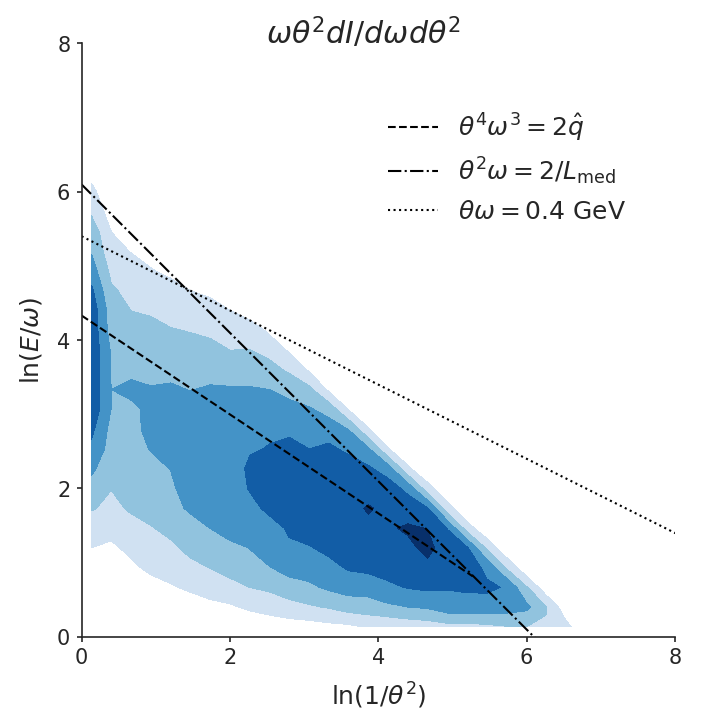
\includegraphics[width=.5\textwidth]{lund-vac.png}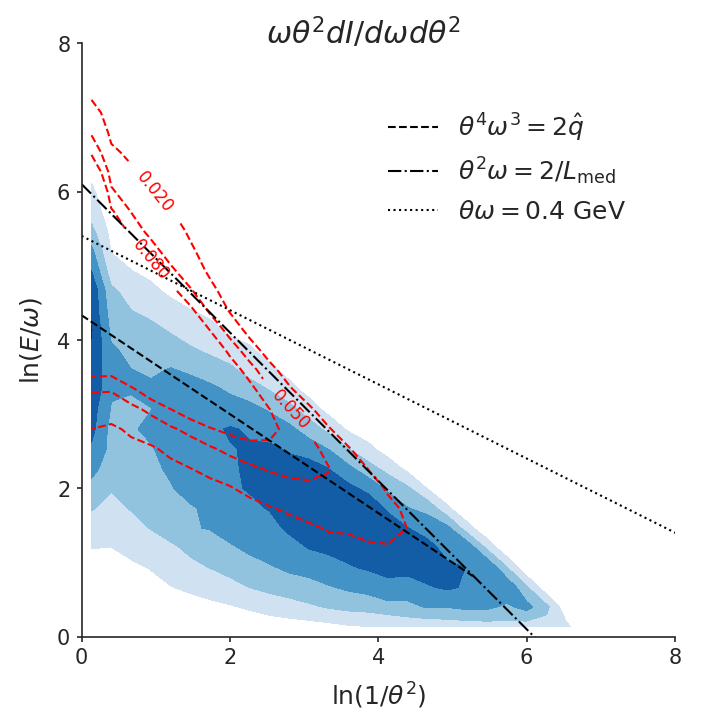
\includegraphics[width=.5\textwidth]{lund-med.png}
\caption{}
\label{fig:lund}
\end{figure}

Concluding this section, the realm of the transport equation and the DGLAP evolution is separated when the parton virtuality is comparable to the acquired transverse momentum broadening within the formation time.
High virtuality evolution is approximated as unmodified, while low virtuality evolution is terminated and replaced by the medium-induce processes via the transport evolution. 
Using the Lund diagram to visualize the simulation, medium-induced and vacuum branchings occupy relatively separated region of the phase-space, though smeared by a large fluctuation.
This procedure is, of course, only viable if we initialize the simulation with parton shower event generator.
We are not able to do such a separation using heavy quark spectra obtained from FONLL.

\section{Particles coupled to an evolving medium}
The coupling between hydrodynamics and hard parton transport often require a switching of different reference frames, as velocity of the medium local-rest-frame relative to the lab frame is function of space-time.

\paragraph{For diffusion dynamics} The diffusion equations are most easily  written in the local-rest-frame of the medium.
Given a particle's four momentum in the lab frame ($p_{L}^\mu$), one first boost it into the medium local-rest-frame ($p_{M}^\mu$),
\begin{eqnarray}
p_{M}^\mu &=& L^\mu_\nu(\vec{\beta}) p_{L}^\nu\\
L^\mu_\nu &=& 
\begin{bmatrix}
\gamma & -\gamma\vec{\beta}\\
-\gamma\vec{\beta} & \mathbb{1} + \frac{\gamma^2}{\gamma+1}\vec{\beta}\vec{\beta}
\end{bmatrix}
\end{eqnarray}
where $\vec{\beta}$ is the velocity of the fluid cell relative to the lab frame, and $L^\mu_\nu$ is the Lorentz transformation.
One needs to be careful with that the time step in the fluid rest frame $\Delta t_{M}$ is different from the one in the lab frame $\Delta t_{L}$.
Consider the particle trajectory $\Delta x_{L}^\mu$ within $\Delta t_{L}$ observed in the lab frame and boost it into the medium frame,
\begin{eqnarray}
\Delta x_{L}^\mu = \frac{p_{L}^\mu}{E_L} \Delta t_{L} \xrightarrow{\textrm{boost}} \Delta x_{M}^\mu = \frac{L^\mu_\nu(\mathbf{v}_{M}) p_{L}^\nu}{E_L} \Delta t_L = \frac{p_{M}^\mu}{E_L} \Delta t_L
\end{eqnarray}
Now compare the time-component of the equation, one get the time step in the medium frame is related to the lab frame step by the ratio between the energy of the particle in the two reference frames,
\begin{eqnarray}
\Delta t_M = \frac{E_M}{E_L} \Delta t_L
\end{eqnarray}
Once the momentum is updated in the medium frame to become $p'_M$, it is boosted back to the lab frame,
\begin{eqnarray}
x'^{\mu} &=& x^{\mu} + \frac{p_{L}^\mu}{E_L} \Delta t_{L} \\
p_{L}^{'\mu} &=& L^\mu_\nu(-\vec{\beta}) p_{M}^{'\nu}
\end{eqnarray}
where we have chosen to update position before the update of the momentum.

The choice of $\Delta t_L$ is also tricky. 
A most straightforward uniform time step for all the particles is not the optimal choice.
This is because that relativistic hydrodynamics for heavy-ion collision is often solved in the $(\tau,x,y,\eta_s)$ coordinates, and the hydrodynamic field is propagated from one constant proper time $\tau = \sqrt{t^2 - z^2}$ to the next.
There are two consequences if we choose the same $\Delta t_L$ for all particles:
\begin{itemize}
\item[1.] Different particles will be at different proper times $\tau$ at a constant $t$. It requires the program to load the entire hydrodynamic temperature and velocity history into the memory, which can be a potential problem for 3+1 D hydro simulation (the memory consumption for boost-invariant hydrodynamics is not critical).
\item[2.] The time step in medium-rest-frame for particles at large space-time rapidity would be too small.
\end{itemize}
For these practical reasons, we choose to propagate particles with a constant proper-time step $\Delta \tau$. 
As a result, the time step in the lab frame is different for each particle, depending on its location and momentum, and is solved by,
\begin{eqnarray}
\Delta \tau = \sqrt{(t+\Delta t_L)^2 - (z+v_z \Delta t_L)^2} - \sqrt{t^2 - z^2}.
\end{eqnarray}
This is (keeping the positive solution),
\begin{eqnarray}
\Delta t_L(p, x) = \frac{-(t-z v_z) + \sqrt{(t-z v_z)^2 - (1-v_z^2)(\Delta \tau^2 + 2\sqrt{t^2 - z^2}\Delta \tau )}}{2(1-v_z^2)}
\label{eq:dt-transformation}
\end{eqnarray}
This adaptive time step propagate a particle between constant proper-time hyper-surface, therefore only two steps of hydrodynamic information needs to be loaded into memory at a time.
Also $\Delta t_L$ becomes larger for forward/backward particles.

\paragraph{For matrix-element scattering} The situation for matrix-element scatterings is more complicated.
Because the initial state of scattering is straightforwardly sampled in the medium local-rest-frame, but the full final state is most efficiently sampled in the center-of-mass frame of the few-body collisions.
The center-of-mass velocity relative to the local-rest-frame is,
\begin{eqnarray}
\vec{\beta}_{C} = \frac{\sum_{i\in \textrm{IS}} \vec{p}_i}{\sum_{i\in \textrm{IS}} E_i}
\end{eqnarray}
where ``IS'' stands for the initial state.

\begin{itemize}
\item[1.] For each hard parton, determine $\Delta t_L$ with equation \ref{eq:dt-transformation}.
\item[2.] Boost the particle to the medium rest-frame and sample the scattering rate $\Delta t_M R$ channel, and then sample the medium parton(s) that forms the scattering initial state with the hard parton.
\item[3.] In the CoM frame of the initial state, sample the final state particles.
\item[4.] Boost back the final state particles to the medium rest frame.
\item[5.] Boost back to the lab frame.
\end{itemize}

\section{Heavy-flavor hadronization and hadronic stage}
At a temperature around $T_c$, light hadrons can be sampled from the hydrodynamics energy momentum tensor statistically.
For hard partons that stays off equilibrium, one needs a more microscopic implementation of the hadronization.
Below $T_c$, the hadronic system is also dense enough for the heavy hadron to interact and contribute to the low-$p_T$ $v_2$ of D-meson, though the hadronic interactions are not analyzed so extensively as the QGP interaction.

\subsection{The ``sudden" approximation of hadronization} 
The hadronization model for the heavy flavor is the simulation is implemented by [].
It combines the fragmentation of heavy quark at high momentum and the recombination with medium partons into hadrons at low momentum.

The hadronization is treated to be instantaneous on an isothermal hypersurface.
This ``sudden'' approximation certainly has certain drawbacks.
First, hadronization is a long distance process. 
In the rest frame of the heavy flavor, it takes time scale $1/\Lambda_{QCD}$. 
With a large boost factor $E/M_{\textrm{hadron}}\sim E/M_{\textrm{heavy quark}}$, the formation time of the heavy hadron can be comparable to macroscopic length scales.
For example, for a moderate $E=10$ GeV charm quark $M=1.3$ GeV, this time is estimated to be $8$ fm/c, which is certainly not a sudden process considering the hydrodynamic stage only last for $O(10)$ fm/$c$.
Second, an instantaneous recombination process breaks energy conservation and detailed balance, as will be shown below.
To solve these problems, one really needs a dynamical modeling of the hadronization physics in the future,
which is already a hard problem in the vacuum.

\paragraph{Fragmentation} 
In high energy electron-positron collision and proton-proton collision, high momentum heavy quark hadronizes through the fragmentation mechanism.
The energetic heavy quark produces a bunch of hadrons with a heavy hadron that carries a certainty fraction of the origin quark energy $z = p_H/p_Q$.
The probability distribution of $z$ is known as the fragmentation function $D(z)$, and can be measured in, e.g., electron-positron collier.
There are different parametrizations for $D(z)$ and here the Peterson parametrization that is designed for heavy quark is used,
\begin{eqnarray}
D(z) \propto \frac{1}{z(1-\frac{1}{z} - \frac{\epsilon}{1-z})^2}
\end{eqnarray}
where $\epsilon$ is a parameter that scales as $m_Q^{-2}$ ($\epsilon_c \approx 0.05, \epsilon_b \approx 0.006$).

\paragraph{Recombination}
It was known already in proton-proton collision that heavy quark can hadronize into mesons by the recombination with a light anti-quark in the proton remnant [].
In a heavy-ion collision, recombination mechanism can play an important row for low transverse momentum heavy flavors, given the abundance of the medium thermal partons.
Early study in the nuclear collisions [] assumes that the recombination probability can be computed from the wave function overlap between initial state partons and final state mesons or baryons, with the momentum of the medium parton integrated over the thermal distribution.
The model we used is an implementation of this idea for the charm and bottom sector [],
\begin{eqnarray}
\frac{dP_M(p', p)}{dp'^3} &=& \int dk^3 n_{\bar{q}}(k) W_{M}(p, k)\delta^{(3)}(\vec{p}'-\vec{p}-\vec{k}), \label{eq:meson_recombine}\\
\frac{dP_B(p', p)}{dp'^3} &=& \int dk_1^3 dk_2^3 n_{\bar{q}}(k_1)  n_{\bar{q}}(k_2) W_{B}(p, k_1, k_2)\delta^{(3)}(\vec{p}'-\vec{p}-\vec{k}_1 - \vec{k}_2), \label{eq:baryon_recombine}.
\end{eqnarray}
On the left are the differential probability for a heavy quark with momentum $p$ to hadronize into a heavy meson (first line) or a heavy baryon (second line) with momentum $p'$ through recombination.
They are equal to an integration of light quark(s) / anti-quark momentum  of the production of baryon /meson Wigner function $W$ times the thermal distriubtion function, subjected to three-momentum conservation.
It is evident that the energy conservation is not imposed in the instantaneous $2\rightarrow 1$ coalescence approach.
The quark / anti-quark distribution function is the Fermi-Dirac one, neglecting chemical potential, 
\begin{eqnarray}
n = \frac{g_q V}{e^{\beta p\cdot u} + 1}
\end{eqnarray}
with $u$ the fluid velocity and the $p$ the four momentum of the light quark / anti-quark.
$g$ is the degeneracy of the quark, and $V$ is a test volume that will eventually be canceled by the normalization factor in the the Wigner function.
As a remark, we have assumed in the transport model that medium partons are massless because the thermal masses are higher effects for energy loss; but for recombination into bound states near $T_c$, it is important to use non-perturbative constituent masses of light quarks $m_u = m_d = 300$ MeV and $m_s = 475$ MeV.

Regarding the meson wave-function, there has been efforts using Dirac equation and to obtain a more realistic wave-function for different state of heavy mesons.
But the current model uses parametrized Gaussian wave-function for simplicity,
\begin{eqnarray}
\phi_M(\vec{r}) &=& \left(\frac{1}{\pi \sigma^2}\right)^{3/4} e^{-\frac{r^2}{2\sigma^2}}
\end{eqnarray}
The $\sigma$s are related to the reduced mass of the two body system $\mu = m_1 m_2/(m_1+m_2)$ and the frequencty of the  two-body potential $\omega$ by $\sigma = 1/\sqrt{\mu \omega}$.
These frequencies is estimated from the charge radius of different heavy mesons: $0.106$ GeV for charmed hadron and $0.059$ GeV for the bottom mesons.
The Wigner function is defined in terms of the relative distance $\vec{r}$ and relative momentum $\vec{q}$ between the quark and anti-quark,
\begin{eqnarray}
W_M(\vec{r}, q^2) &=& g_M \int d^3 \vec{a} e^{-i\vec{q}\cdot \vec{a}} \phi_M(\vec{r}+\vec{a}/2) \phi_M^*(\vec{r}-\vec{a}/2) \\
\vec{q} &=& \frac{E_2\vec{p}_1 - E_1\vec{p}_2}{E_1+E_2}.
\end{eqnarray} 
Averaging over the light quark's positions,
\begin{eqnarray}
W_M(q^2) &=& \frac{g_M}{V} (2\sqrt{\pi}\sigma)^3 e^{-\sigma^2 q^2},
\end{eqnarray}
which is the quantity needed in equation \ref{eq:meson_recombine},
\begin{eqnarray}
\frac{dP_M(p',p)}{dp'^3} &=& \int dk^3 \frac{g_q g_M}{e^{\beta p\cdot u} + 1} (2\sqrt{\pi}\sigma)^3 e^{-\sigma^2 q^2} \delta^{(3)}(\vec{p}'-\vec{p}-\vec{k}),
\end{eqnarray}
where the test volume in the distribution function has been canceled by the one in the Wigner function.

The same procedure applies to heavy baryon, with the three-body Wigner function in the Gaussian approximation as,
\begin{eqnarray}
f_B^W(q_1^2, q_2^2) = \frac{N g_B}{V^2} (2\sqrt{\pi\sigma_{1,2}\sigma_{12,3}})^6 e^{-q_{1,2}^2 \sigma_{1,2}^2 - q_{12,3}^2 \sigma_{12,3}^2}.
\end{eqnarray}
With the relative momenta defined as,
\begin{eqnarray}
\vec{q}_{1,2} &=& \frac{E_2 \vec{p}_1 -E_1\vec{p}_2}{E_1+E_2}\\
\vec{q}_{12,3} &=& \frac{E_3 (\vec{p}_1+\vec{p}_1) - (E_1+E_2)\vec{p}_3}{E_1+E_2 + E_3}
\end{eqnarray}
And the $\sigma$ related to the frequency and masses by,
\begin{eqnarray}
\sigma_{1,2}^{-1} &=& \sqrt{\omega \frac{m_1m_2}{m_1+m_2}}\\
\sigma_{12,3}^{-1} &=& \sqrt{\omega \frac{(m_1+m_2)m_3}{m_1+m_2+m_3}}
\end{eqnarray}

To synthesis these two competing mechanisms of hadronization, one first samples the recombination probability in equations \ref{eq:meson_recombine} and \ref{eq:baryon_recombine} and determines whether the heavy quark coalesces with the medium partons. 
If not, its hadronization will be handled by the Pythia fragmentation routine with the Peterson fragmentation function.

\subsection{Hadronic rescattering}
Currently, the hadronic rescattering of charmed mesons with $\pi$ and $\rho$ mesons are included the UrQMD frame as the light hadrons. 
These cross-sections are obtained from [].
Hadronic cross-section of the charmed baryons and bottom hadrons are not included.

One modification is made to the UrQMD heavy-flavor sector that the back reaction from heavy flavor mesons to light sector is turned-off. 
This is done by resetting the light scattering partner's four momentum back to its initial value.
This is to the same level of approximation of the linearized transport equation in the QGP phase, and allows for an easy oversampling of the number of heavy flavor particles to obtain better statistics.

\section{Benchmark calculation of observables}
In the last section of this chapter, we provide a benchmark calculation of this open-heavy flavor simulation framework to experimental data, systematic calibration of model parameters and uncertainties will be discussed in the next to chapters.

\subsection{Open heavy flavor observables}
The ground states $D^0, \bar{D}^0, D^{\pm}, B^{\pm}, D_s^{\pm}, B_s^{\pm}$ mesons and the excited states $D^{*\pm}$ can be measured in the experiments.
The $D_s^{\pm}$ is interested as it contains the information of the strangeness enhancement in the thermal medium.
Currently, we only focus on the non-strange D and B mesons.

\paragraph{Nuclear modification factor}
The nuclear modification factor is defined as the ``normalized'' ratio of the heavy flavor yield in nuclear collision of a certain centrality to that in the proton-proton collision,
\begin{eqnarray}
R_{AA}(y, p_T) = \frac{\frac{dN_{AA}}{dy dp_T}}{\langle N_{\textrm{coll}}\rangle \frac{dN_{pp}}{dy dp_T}} = \frac{\frac{dN_{AA}}{dy dp_T}}{\langle T_{AA} \rangle \frac{d\sigma_{pp}}{dy dp_T}} .
\end{eqnarray}
The ``normalization'' refers to scale the proton-proton yield by the average number binary nucleon inelastic collision so that one expects an unity $R_{AA}$ in the absence of nuclear effects.
The number of binary collision is sometimes replaced by the average nuclear overlapping function $\langle N_{\textrm{coll}}\rangle = \langle T_{AA} \rangle /\sigma_{pp}^{\textrm{inel}}$, and the yield is replaced by the inclusive cross-section for the proton-proton collision $\frac{dN_{pp}}{dy dp_T}\rightarrow \frac{d\sigma_{pp}}{dy dp_T}$.
These two expressions are equivalent.

The reason that we put a quotation mark on the work ``normalization'' is to remind the readers that $N_{\textrm{coll}}$ is not a directly observed quantity. 
It has to be estimated in a model-dependent way.
Experiments uses slightly different versions of the Monte-Carlo Glauber model (introduced in chapter \ref{chapter:simulation}) to determine the relation between the average $N_{\textrm{coll}}$ and centrality.
In the \trento\ model, we also found that the relation of $\langle N_{\textrm{coll}} \rangle$ versus centrality is sensitive to the nucleon shape, e.g., a black disk nucleon versus a Gaussian nucleon.
Ultimately, whether the normalization factor is correct has to be validated by the production of colorless probe such as $Z$-boson that does not interact with the hot medium.
Recent measurements of the $Z$-boson production has reached a precision higher than the current estimated uncertainty of the Glauber model, and can be used for future fine tune of the initial nuclear geometry model.

\paragraph{Momentum anisotropy}
The momentum anisotropy $v_n$ measures the azimuthal anisotropy relative to the flow vector of the bulk medium.
Heavy flavors momentum anisotropy at high-$p_T$ is thought to be the result of aisntorpic energy loss, because hard partons emitted in the short axis direction losses less energy than those emitted from the long axis direction on average.
At low momentum, the momentum anisotropy has a flow origin that heavy quark interacts so frequently with the medium and tends to catch up with the flow velocity of the medium.

We used the so called $Q$-vector method to compute $v_n$ from two-particle correlation,
\begin{eqnarray}
v_n\{2\}(p_T) = \frac{\mathfrak{Re}\langle d_n\{2\} \rangle}{\langle c_n\{2\}\rangle}.
\end{eqnarray}
$c_n$ is the event-wise two particle correlation of $N$ reference particles (REF, the bulk medium) within a certain kinematic range,
\begin{eqnarray}
c_n &=& \frac{|Q_n|^2 - N}{N(N-1)},  \\
Q_n &=& \sum_{i=1}^N e^{i n \phi},
\end{eqnarray}
and the event average ($\langle\cdots\rangle$) is weighted by $N(N-1)$.
$d_n$ is the correlation of $Q$-vectors between the $M$ particles of interest (POI, in this case the heavy flavors) and the reference particles,
\begin{eqnarray}
d_n &=& \frac{q_n Q_n^* - m}{MN-m},  \\
q_n &=& \sum_{j=1}^M e^{i n \phi},
\end{eqnarray}
and $m$ is the number of POI that is also REF to subtract auto correlations. 
And its event average is weighted by $MN-m$.

\paragraph{Event-shape engineering on heavy-flavor observables}
Event-shape engineering is a more recent idea to look at the detailed response of the hard sector, varying the properties of the medium evolution.
Experimentally, an ensemble of events belongs to a certain centrality class is further classified according to its ``event shape'', measured by $q_2$,
\begin{eqnarray}
q_2 = \frac{|Q_2|}{\sqrt{N}}.
\end{eqnarray}
Due to event-by-event geometry fluctuation, the event shape in the a given centrality class can be vary a lot.
The ALICE experiment then measures the D meson $v_2$ with events having the $20\%$ largest $q_2$ and events with the $60\%$ smallest $q_2$.
And found a large separation between the the resulting $v_2$ with biased selected events compared to the $v_2$ calculated from unbiased events.
This measurement quantifies the response of hard probe to the event geometry fluctuation, that may provide sensitivity to the way a transport code handles a fluctuating medium.

\subsection{A first comparison to data}
We do not intend optimize all the parameters in the model in this first comparison to data, but uses reasonable guess of the parameters to understand the model.
The TRENTo parameters and the hydrodynamic transport coefficients are obtained from [].
The heavy quark flavor starts to lose energy from $0.6$ fm/$c$, and the matching condition between the vacuum-like radiation and the medium-induced radiation is $k_\perp^2 = \Delta k_\perp^2$.
We used only leading order contribution from the weakly coupled theory, and tried both fixed coupling and running coupling.
The default switching scale between a large-$Q$ scattering small-$Q$ is $Q_{\textrm{cut}}^2 = 4 m_D^2$ and we the observables at relatively high-$p_T$ is not sensitive to this scale.

\paragraph{Fixed coupling} First, we compute with fixed coupling constant $\alpha_s = 0.2, 0.3, 0.4$.
\begin{figure}
\centering
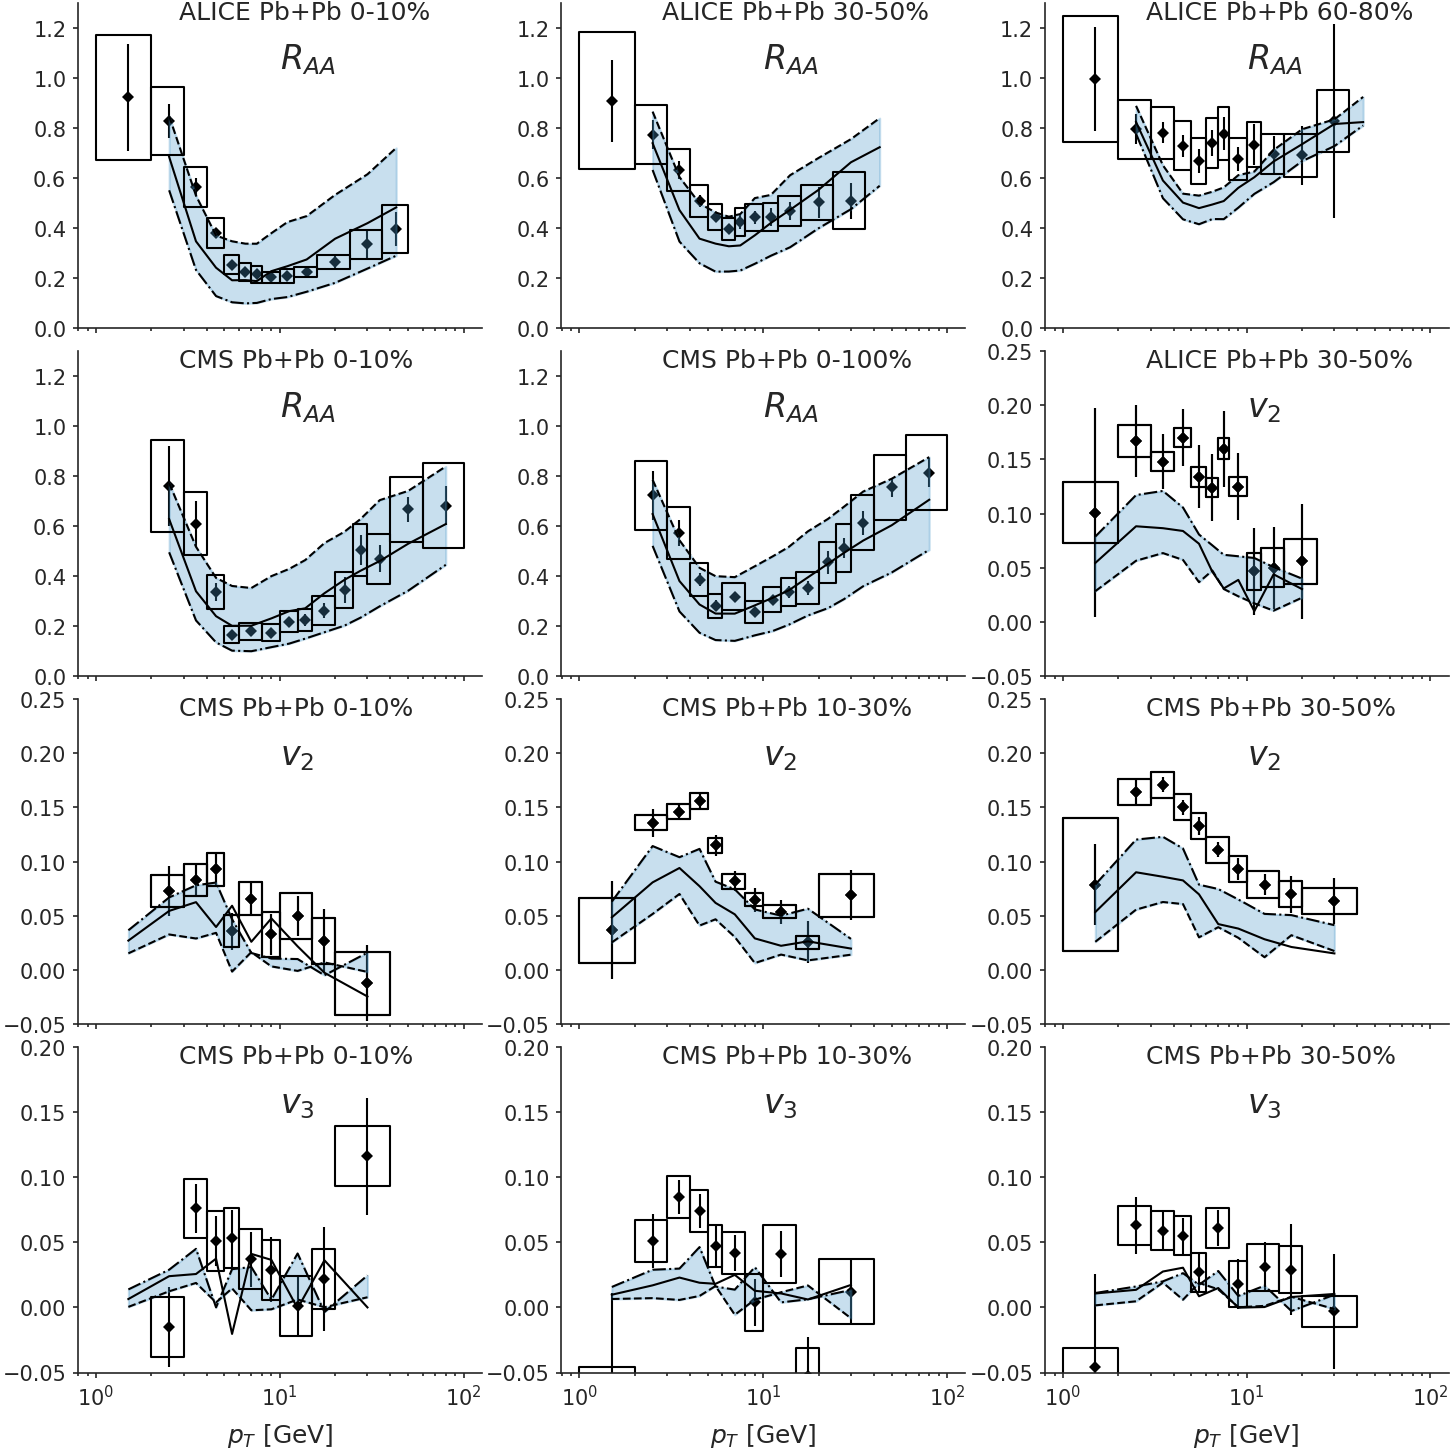
\includegraphics[width=\textwidth]{New-analysis/fix_alphas.png}
\caption{}
\label{fig:new:fix-a}
\end{figure}

\paragraph{Running coupling}
\begin{figure}
\centering
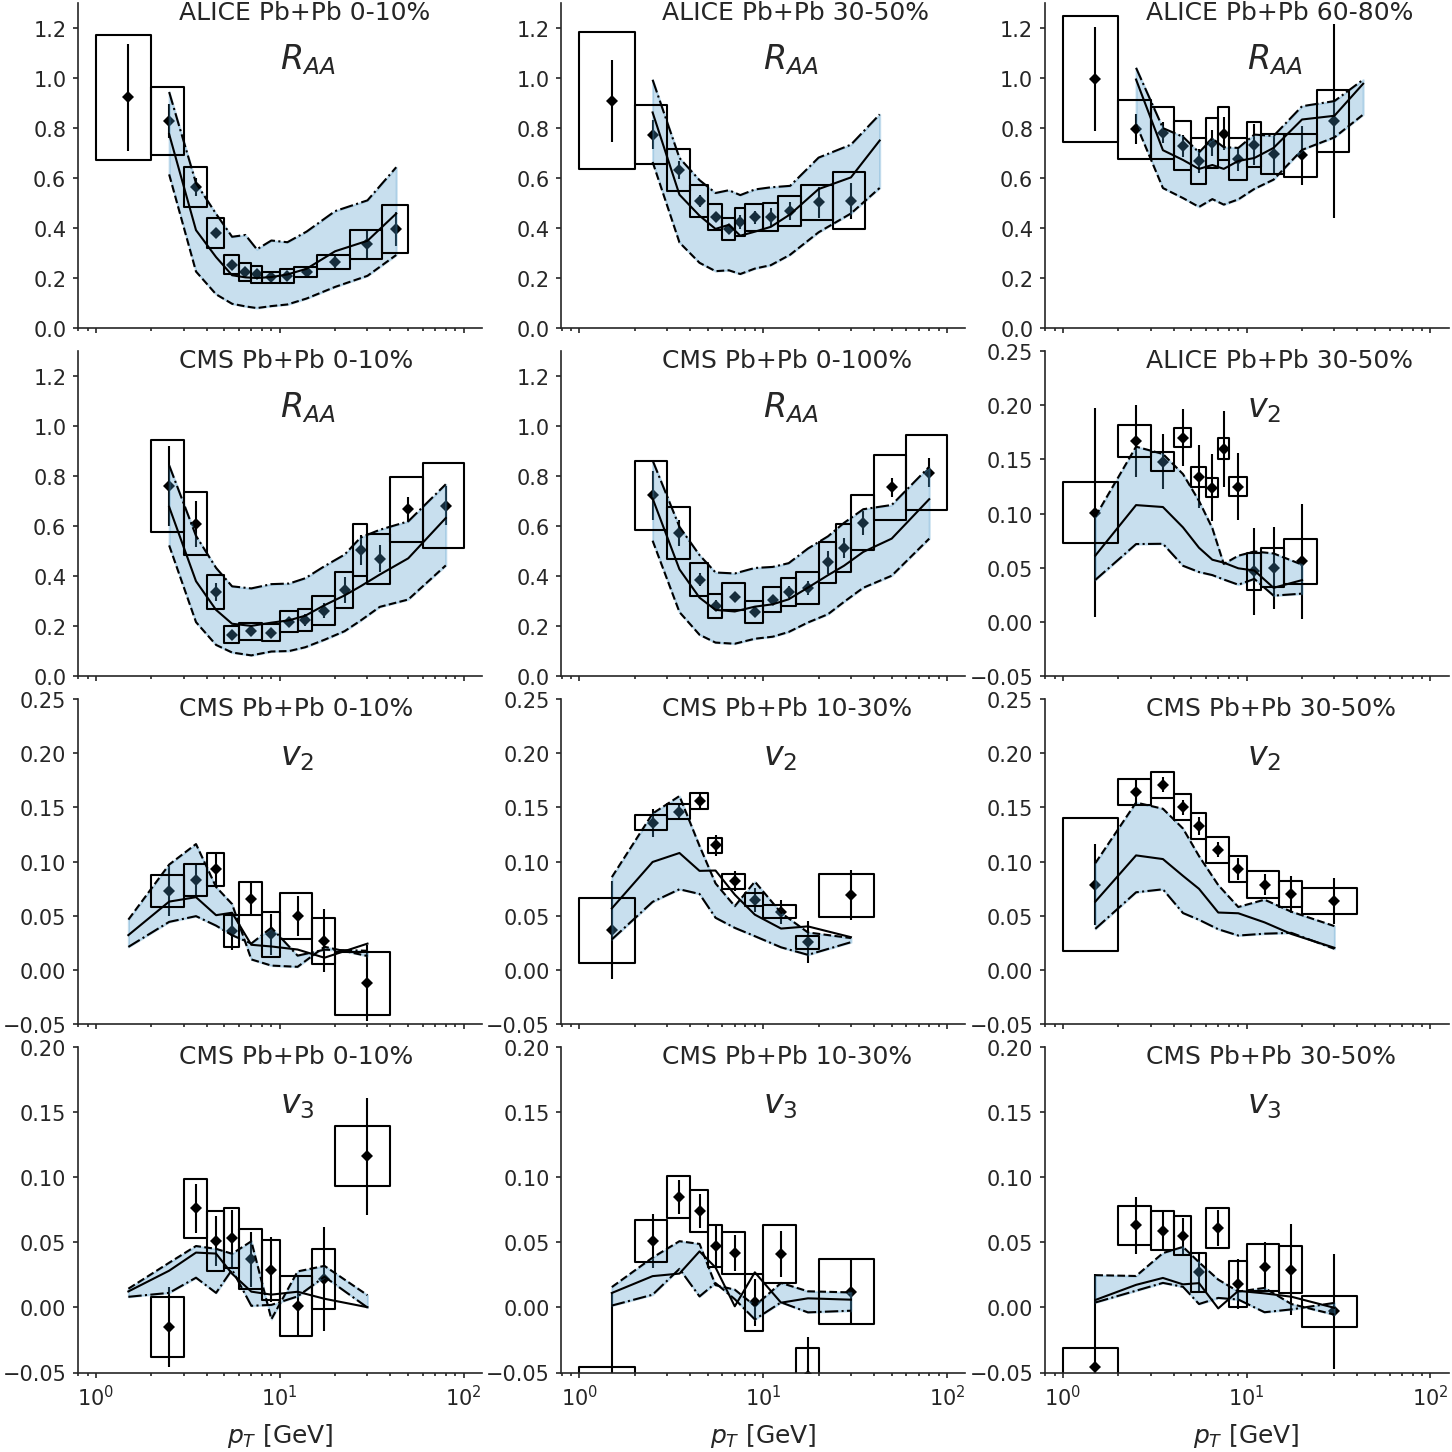
\includegraphics[width=\textwidth]{New-analysis/run_alphas.png}
\caption{}
\label{fig:new:run-a}
\end{figure}

\paragraph{Switching scale dependence}
\begin{figure}
\centering
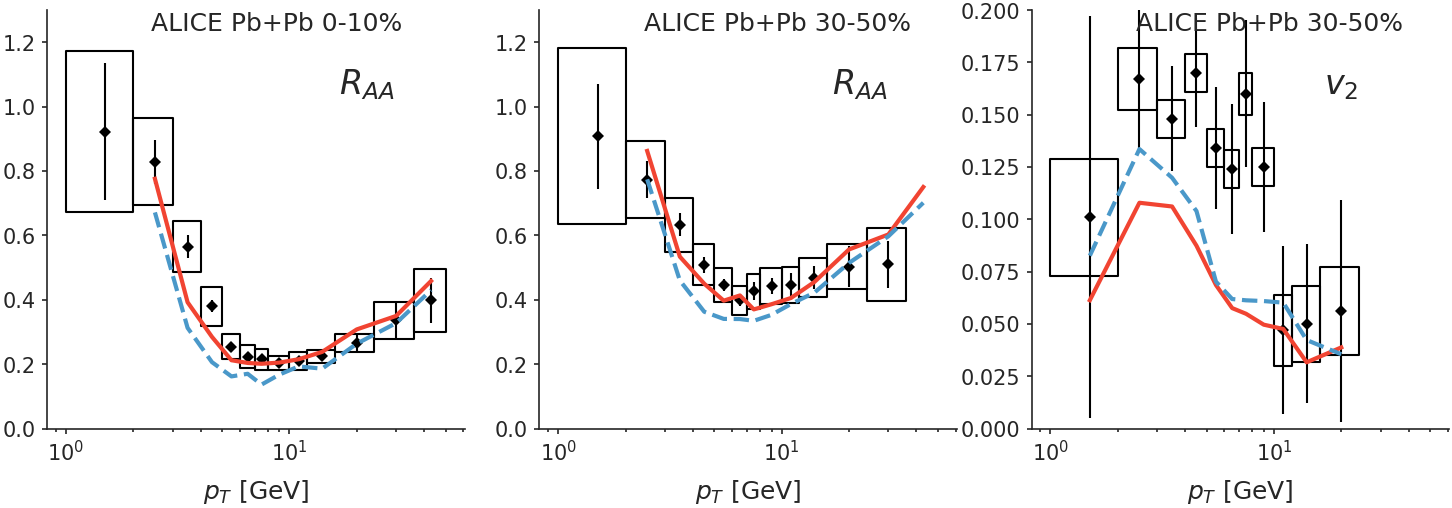
\includegraphics[width=\textwidth]{New-analysis/run_alphas_cut.png}
\caption{}
\label{fig:new:run-a}
\end{figure}

\paragraph{Vacuum-radiation matching scale dependence}
